%!TEX root = main.tex
\chapter{Anhang}


%!TEX root = main.tex

\section*{Python Cheat Sheet}
\subsection*{Numerisches,Arrays und Plots}
\begin{table}[H]
    \centering
    \begin{tabular}{|l|l|p{7cm}|}
        \hline
    \textbf{Befehl} & \textbf{Beispiel} & \textbf{Kommentar} \\ \hline
    
    \texttt{\%pylab} & \texttt{\%pylab} & Schneller import von üblichen paketen (\texttt{matplotlib} und \texttt{numpy}). \\ \hline
    \texttt{zeros()} & \texttt{x = zeros(5)} & Generierung eines arrays, mit nullen befüllt. \\ \hline
    \texttt{linspace()} & \texttt{x = linspace(0,1, 5)} & Generierung eines arrays, zahlen linear zwischen Argument 1 und 2 erzeugt, Anzahl der zahlen bestimmt durch argument 3. \\ \hline
    \texttt{plot()} & \texttt{plot(x,y)} & Line-plot erzeugen.  \\ \hline
    \texttt{clf()} & \texttt{clf(x,y)} & Clear figure. Aktuellen plot löschen.  \\ \hline
    \texttt{scatter()} & \texttt{scatter(x,y)} & Scatter Plot erzeugen. \\ \hline
    \texttt{stem()} & \texttt{stem(x,y)} & Stem Plot erzeugen. \\ \hline

    \texttt{[]} & \texttt{x[5] = 3} & Element aus array anzeigen holen oder bearbeiten. Im Bsp. wird dem 6. Element des array \texttt{x} der Wert 3 zugewiesen. \\ \hline
    \texttt{random.random()} & \texttt{random.random(50)} & Erzeuge 50 gleichverteilte Zufallszahlen im halboffenen Intervall $[0.0, 1.0)$. \\ \hline
    \texttt{**} & \texttt{x**3} & Exponenzieren. Im Bsp.: $x^3$. \\ \hline

    \end{tabular}
\end{table}

\subsection*{Symbolische Mathematik}
\begin{table}[H]
    \centering
    \begin{tabular}{|l|l|p{7cm}|}
        \hline
    \textbf{Befehl} & \textbf{Beispiel} & \textbf{Kommentar} \\ \hline
    
    \texttt{import sympy as sp} & \texttt{import sympy as sp} & Import des \texttt{sympy} Pakets für symbolische Berechnungen. \\ \hline
    \texttt{sp.roots()} & \texttt{x = sp.roots(p)} & Findet die Nullstellen des polynoms \texttt{p}. \\ \hline
    

    \end{tabular}
\end{table}


\section*{Griechisches Alphabet}\label{sec:greekAlph}
\begin{table}[H]
    \centering
    \begin{tabular}{|c|c|c|p{7cm}|}
        \hline
        \textbf{Buchstabe} & \textbf{Kleinbuchstabe} & \textbf{Großbuchstabe} & \textbf{Typische Verwendung im Audio-Bereich} \\
        \hline
        Alpha   & $\alpha$ & $A$ &  Schallabsorptionsgrad, Allg. Winkel \\
        \hline
        Beta    & $\beta$  & $B$ & Dämpfungsfaktor, Ausbreitungskonstante \\
        \hline
        Gamma   & $\gamma$ & $\Gamma$ & Reflexionskoeffizient, spezifische akustische Impedanz \\
        \hline
        \rowcolor{tableHighligh}
        Delta   & $\delta$ & $\Delta$ & Impuls, Änderung einer Größe,Schalldissipationsgrad \\
        \hline
        Epsilon & $\epsilon, \varepsilon$ & $E$ & Permittivität, Fehlerterme bei Näherungen \\
        \hline
        Zeta    & $\zeta$  & $Z$ & eher selten im Audio-Bereich \\
        \hline
        Eta     & $\eta$   & $H$ & Wirkungsgrad, Viskositätseffekte in der Fluidakustik \\
        \hline
        Theta   & $\theta$ , $\vartheta$ & $\Theta$ & manchmal Phasenwinkel, Winkelposition, Temperatur (Akustik) \\
        \hline
        Iota    & $\iota$  & $I$ & Selten im Audio-Bereich verwendet \\
        \hline
        Kappa   & $\kappa$ & $K$ & Wellenzahl, Wärmeleitfähigkeit \\
        \hline
        \rowcolor{tableHighligh}
        Lambda  & $\lambda$ & $\Lambda$ & Wellenlänge, Eigenwerte in der Modalanalyse, Lamé Konstante I \\
        \hline
        Mu      & $\mu$    & $M$ & Mikro-Präfix (z.B. Mikrosekunden), Durchschnitt, manchmal Poissonzahl, Lamé Konstante II \\
        \hline
        \rowcolor{tableHighligh}
        Nu      & $\nu$    & $N$ & Frequenz (!), Anzahl der Modi, Poissonzahl \\
        \hline
        Xi      & $\xi$    & $\Xi$ & Selten im Audio-Bereich verwendet \\
        \hline
        Omikron & $o$      & $O$ & Selten im Audio-Bereich verwendet \\
        \hline
        \rowcolor{tableHighligh}
        Pi      & $\pi$    & $\Pi$ & Kreiszahl, Produkte \\
        \hline
        \rowcolor{tableHighligh}
        Rho     & $\rho$, $\varrho$   & $P$ & Dichte (-> Akustik), spezifischer Widerstand,  Schallreflexionsgrad \\
        \hline
        \rowcolor{tableHighligh}
        Sigma   & $\sigma$ & $\Sigma$ & Standardabweichung, Summation von Größen \\
        \hline
        \rowcolor{tableHighligh}
        Tau     & $\tau$   & $T$ & Zeitkonstante, Verzögerungszeit, Schalltransmissionsgrad \\
        \hline
        Ypsilon & $\upsilon$ & $\Upsilon$ & Selten im Audio-Bereich verwendet \\
        \hline
        \rowcolor{tableHighligh}
        Phi     & $\phi$, $\varphi$   & $\Phi$ & Phase \\
        \hline
        Chi     & $\chi$   & $X$ & Selten im Audio-Bereich verwendet \\
        \hline
        Psi     & $\psi$   & $\Psi$ & Wellenfunktion in der Quantenmechanik daher manchmal Wellenpakete. (aber eher selten im Audio) \\
        \hline
        \rowcolor{tableHighligh}
        Omega   & $\omega$ & $\Omega$ & Kreisfrequenz, Ohm, Normierte Frequenz \\
        \hline
    \end{tabular}
    \caption{Griechisches Alphabet in Mathematik und Audio-Anwendungen. Besonders 'Audio relevante' Buchstaben hervorgehoben.}
\end{table}


\section*{Formelsammlung}\label{sec:formelsam}

\mygrid{Funktionen}{
    $-sinx = sin(-x)$ & $cos(-x) = cosx$ \\ \hline
    $log_a x = \frac{log_b x}{log_b a}$
}


\mygrid{Physik}{
    $F = ma$ & $p = mv$ \\ \hline
    % $v_f = v_i + at$ & $a = \frac{v_f - v_i}{t}$ & $\Delta p = F \Delta t$ \\ \hline
        \resizebox{0.2\textwidth}{!}{ % Scale to 30% of the text width
        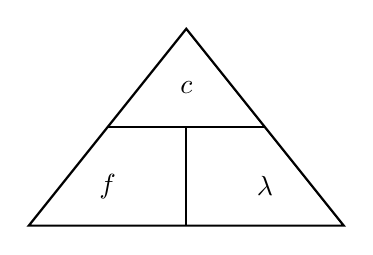
\begin{tikzpicture}
            % Draw the triangle
            \draw[thick] (0, 0) -- (2, 2.5) -- (4, 0) -- cycle; % Triangle vertices

            % Shortened horizontal split (middle)
            \draw[thick] (1, 1.25) -- (3, 1.25); % Horizontal line in the middle

            % Vertical splits (lower half)
            \draw[thick] (2, 0) -- (2, 1.25); % Vertical line in lower half

            % Add the letters
            % Upper field
            \node at (2, 1.75) { $c$}; % Centered in the upper field, smaller font

            % Lower left field
            \node at (1, 0.5) { $f$}; % Centered in the lower left field, smaller font

            % Lower right field
            \node at (3, 0.5) { $\lambda$}; % Centered in the lower right field, smaller font
        \end{tikzpicture}
    }
}

% \vspace{1em} % Adjust space between grids
\vspace{-1em} % Adjust space between grids

% \mygrid{Geometry Equations}{
%     a^2 + b^2 = c^2 & \text{Area} = \pi r^2 & V = lwh \\
%     A = \frac{1}{2}bh & s = \frac{n(n + 1)}{2} & P = 2(l + w)
% }

% \vspace{1em}


\mygrid{Analysis}{
    $\int uv' = uv - \int vu'$ & $(u\cdot v)' = u'v + uv'$ \\ \hline
    $\frac{d}{dx}(a^x) = a^x \cdot ln(a)$ \\ \hline
    $\int_a^b f(x) \, dx = F(b) - F(a)$ & $\lim_{x \to 0} \frac{\sin x}{x} = 1$ \\ \hline
    $e^{i\pi} + 1 = 0$ & $\frac{d}{dx}(e^x) = e^x$ & $\int e^x \, dx = e^x + C$

}

% $\frac{dy}{dx} = f'(x)$ 

\mygrid{Integrale}{
    $\int sin(x) dx= -cos(x)$ & $\int cos(x) dx= sin(x)$ \\ \hline
    $\int sin(ax) dx= -\frac{1}{a}cos(ax)$ & $\int cos(ax) dx= -\frac{1}{a}sin(ax)$
}



% \begin{figure}[htbp]
%     \centering
%     \resizebox{0.2\textwidth}{!}{ % Scale to 30% of the text width
%         \begin{tikzpicture}
%             % Draw the triangle
%             \draw[thick] (0, 0) -- (2, 2.5) -- (4, 0) -- cycle; % Triangle vertices

%             % Shortened horizontal split (middle)
%             \draw[thick] (1, 1.25) -- (3, 1.25); % Horizontal line in the middle

%             % Vertical splits (lower half)
%             \draw[thick] (2, 0) -- (2, 1.25); % Vertical line in lower half

%             % Add the letters
%             % Upper field
%             \node at (2, 1.75) { $c$}; % Centered in the upper field, smaller font

%             % Lower left field
%             \node at (1, 0.5) { $f$}; % Centered in the lower left field, smaller font

%             % Lower right field
%             \node at (3, 0.5) { $\lambda$}; % Centered in the lower right field, smaller font
%         \end{tikzpicture}
%     }
%     \label{fig:triangle}
% \end{figure}